\chapter{\label{III-A}Les labyrinthes comme réseaux de données et de liens}
\titreEntete{Les labyrinthes comme réseaux de données et de liens}

%intro
La multiplication des liens et de ceux possibles dans le Web de données entraîne une désorganisation --- aux yeux d'un humain --- des informations et des référentiels dans ce Web de données. Les chemins à emprunter deviennent multiples et provoquent une ivresse de rebonds et d'informations chez l'utilisateur. Les interfaces de visualisation structurent l'ensemble des informations et des liens du Web de données qui est devenu un Web où seule une machine peut se repérer rapidement et naviguer aisément. Du modèle du graphe d'un jeu de données, le Web de données a permis de créer un graphe à l'échelle du Web, accessible par tous et en tous points, depuis n'importe lequel des jeux de données, des référentiels ou des institutions.\\

La notion de graphe, de réseau de données, découle des nombreuses théories d'arbres de classifications et de descriptions des précédents millénaires. La constatation des limites et de l'échec de ces arbres a conduit à la théorisation, puis l'adoption dans le Web de données et par le milieu bibliothéconomique d'abord, du labyrinthe et du modèle-réseau de données. Le lien devenant l'essence-même de ces réseaux de données, de nouveaux types de référentiels ont vu le jour, notamment les hubs de liens qui centralisent les liens et quelques données d'autorités autour d'un même identifiant. Wikidata, d'abord réceptacle structuré des données et des informations des Wikipédias, devient rapidement le hub de liens et d'identifiants le plus utilisé.

\section{\label{III-A-1}Du modèle encyclopédique aux graphes de données}
\titreEntete{Du modèle encyclopédique aux graphes de données}

%intro
Au Moyen-Âge, la dogmatique de l'arbre porphyrien domine. Ce n'est qu'à la Renaissance que le savoir est conçu comme ouvert. L'arbre était pensé selon le monde, pensé lui-même comme un cosmos clos et ordonné; ce même arbre était par ailleurs pensé comme une finitude inaltérable de sphères. Cependant, la pensée de Copernic influe la façon de concevoir le savoir: ce dernier s'efforce de mimer le système planétaire avec ses perspectives variables, des orbites qui deviennent des ellipses, \dots~\\

L'encyclopédie n'est alors plus qu'un amas de connaissances réelles et légendaires; elle devient un index devant décrire le monde et les connaissances, le classifier. La tension pesant sur ce modèle encyclopédique et la quantité infinie de connaissances conduisent à son éclatement au profit d'une forêt où tout est ou peut être relié selon les choix du lecteur.

\subsection{\label{III-A-1-a}Vers les labyrinthes (Renaissance)}
\titreEntete{Vers les labyrinthes}

L'évolution majeure de la Renaissance, faisant suite aux arbres porphyriens puis lulliens, est la nouvelle conception de la structure des éléments du monde: avec Porphyre et ses successeurs, seuls les accidents et les substances sont classifiés; avec la Renaissance, de multiples \index[ref]{typologie@Typologie!index@Index}index d'encyclopédies naissent, accompagnés de réflexions sur les manières d'ordonner le savoir\footnote{\og Nous n'avons plus affaire à une classification de substances et d'accidents, mais à l'index d'une encyclopédie possible et à la tentative de proposer un ordonnancement du savoir\fg{} in \cite{eco_arbre_2010}}. Toute la Renaissance va se concentrer sur cette classification du savoir.\\

La première grande encyclopédie tentant cette classification du savoir est l'\textit{Encyclopaedia septem tomis distincta} de \nP{Johann}{Alsted} en 1620\footcite{alsted_encyclopaedia_1630}: l'index devient la substance-même de cette œuvre. Cette encyclopédie s'inscrit dans la période pansophique de la Renaissance, dans laquelle la réflexion sur une sapience universelle, qui aurait toute l'étendue du savoir, est vive. Si l'arbre de Porphyre voulait simplement être un dictionnaire, un moyen de définir la science, l'index pansophique inspire quant à lui à classifier cette science, et s'éloigne donc du dictionnaire. Cette période pansophique marque bien l'arrêt de la conception hiérarchique du savoir, conçue comme moyen de définir: un autre moyen de décrire ce savoir est possible, en étant plus efficace.\\

Ce nouveau moyen part de la constatation que de multiples chemins peuvent mener à un même savoir. \nP{Francis}{Bacon} le constate, dès 1620, dans l'\textit{Instauratio Magna}\footcite{bacon_instauratio_1620} puis en 1626 dans le \textit{Sylva sylvarum}. Il n'est alors plus question d'arbre unique, mais d'arbres multiples, de labyrinthes avec des chemins ambigus, des ressemblances trompeuses, des spirales et des noeuds complexes\footnote{\og \textit{obliquae et implexae naturarum spirae et nodi}\fg{} in \cite{bacon_instauratio_1620}}. La forêt est un amas de sujets, on n'y trouve plus mais on découvre de nouvelles relations, ce que l'on ne connaissait pas encore et ce que l'on ne cherchait pas. Cependant, la \og tension entre l'arbre et le labyrinthe\fg{}\footcite{eco_arbre_2010} ne faiblit pas: \nP{John}{Wilkins}, à la fin des années 1660, est mis en échec devant ses classifications du savoir qui ne parviennent pas à classer les sujets; une table immense d'index est alors créée pour résoudre cette difficulté.\\

La masse des connaissances à classer étant immense, l'encyclopédie devient un inventaire général des connaissances, incapable de toutes les saisir: \nP{Gottfried Wilhelm}{Leibniz} comprend bien que l'entreprise encyclopédique peut être infinie en raison du nombre de renvois à créer pour s'adapter aux perspectives infinies d'accès à une connaissance. Le labyrinthe prend alors tout son sens: une connaissance est accessible par de multiples points d'accès et ne fait pas partie d'une hiérarchie stricte. Dans le \og Discours préliminaire\fg{} de l'Encyclopédie\footcite{diderot_encyclope_1751}, l'arbre porphyrien et la pensée artistotélicienne sont totalement remis en question. 
\begin{citationLongue}
	Le système général des sciences et des arts est une espèce de labyrinthe, de chemin tortueux, où l'esprit s'engage sans trop connaître la route qu'il doit tenir.\footcite[Discours préliminaire]{diderot_encyclope_1751}
\end{citationLongue}
L'encyclopédie totale et universelle ne pourra jamais voir le jour en raison de son ampleur; elle n'est qu'utopie de la connaissance. Cette utopie, toujours visible aujourd'hui --- les projets \index[ref]{lod@Linked Open Data (LOD)!wikidata@Wikidata}Wikidata ou Wikipédia se veulent le reflet de notre monde ---, ne cessera pas en raison du caractère culturel qu'elle contient: plus que le reflet de notre monde, elle est le reflet de notre culture et de nos cultures spécifiques. L'encyclopédie sert cependant à créer des portions d'encyclopédie, en vue de réaliser des classifications spécifiques à un domaine.

\subsection{\label{III-A-1-b}Des labyrinthes aux graphes}
\titreEntete{Des labyrinthes aux graphes}

L'arrivée de la pensée classificatoire au niveau du labyrinthe a eu lieu à plusieurs reprises, à chaque échec du modèle de l'arbre, notamment avec Porphyre où chaque pas dans l'arbre régénérait sans cesse l'arbre des différences: il n'y a, par conséquent, pas un, mais un nombre infini d'arbres selon leurs contextes. Il existe plusieurs types de labyrinthes dont les trois principaux sont présentés par \nP{Umberto}{Eco}:
\begin{itemize}
	\item Le plus ancien est un labyrinthe classique unicursal, dit de Knossos (\reference{annexe_laby} (\reference{laby_knossos})): la seule possibilité est d'atteindre son centre; en raison de cette caractéristique, il ne peut pas se rapporter à un modèle encyclopédique, ni à un modèle de description des connaissances. En effet, le savoir n'est pas un long couloir dans lequel on accède toujours à la même connaissance.
	\item Le labyrinthe maniériste d'Irrweg permet des choix alternatifs (\reference{annexe_laby} (\reference{laby_irrweg})): toutes les routes mènent à des points morts, sauf un qui est la sortie. Ce labyrinthe est un arbre de décisions, dans lequel les branches sont la représentation des décisions possibles.
	\item Enfin, le labyrinthe qui donne naissance aux réseaux et aux \index[ref]{typologie@Typologie!graphe@Graphe de nœuds et de liens}graphes est le \og labyrinthe réseau\fg{} de \nP{Umberto}{Eco} (\reference{annexe_laby} (\reference{laby_reseau})). Chaque point du labyrinthe peut être connecté à n'importe quel autre point. Cette structure a l'avantage d'être extensible à l'infini, il permet des connexions infinies et des corrections locales qui ne modifient pas le reste du labyrinthe. Évolutif, ce labyrinthe nécessite de l'utilisateur qu'il modifie en permanence l'image qu'il s'en fait: \og Un réseau est un arbre auquel il faut ajouter des couloirs infinis connectant ses noeuds\fg{}\footcite{eco_arbre_2010}.
\end{itemize}
\medskip
Modèle dans lequel les connexions, les liens, sont essentiels, le labyrinthe réseau permet une représentation multidimensionnelle des connaissances et un accès à un point précis par de multiples liens. En 1968, \nP{Ross}{Quillian}\footcite[p.227-270]{minsky_semantic_1968} fait apparaître le réseau sémantique structuré, conçu comme un réseau de nœuds interconnectés\footnote{\og \textit{The memory model consists basically of a mass of nodes interconnected by different kinds of associative links}\fg{} in \cite[p.234]{minsky_semantic_1968}}. Le modèle qu'il décrit part d'un terme souche qui est défini par une série de nœuds, des tokens: ce n'est pour l'instant qu'un arbre. Seulement, les tokens peuvent à leur tour devenir des souches et porter des relations d'association: le réseau est ainsi constamment remodelé et modifié\footnote{\og \textit{Token nodes make it possible for a word's meaning to be built up from other word meanings as ingredients and at the same time to modify and recombine these ingredients into a new configuration}\fg{} in \cite[p.234]{minsky_semantic_1968}}. Ce modèle en réseau permet alors la définition de chaque terme, par ses connexions, avec tous les autres termes; il devient infini et multidimensionnel, non représentable en entier sur un plan bidimensionnel: la complexité du modèle-réseau peut être uniquement traité et compris par une machine. 

%conclu
\bigskip
\bigskip
L'apparition du modèle-réseau, du labyrinthe-réseau, a montré l'importance du lien dès la seconde moitié du \textsc{XX}\textsuperscript{ème}siècle. L'informatique a permis de mettre fin aux structures de connaissances qui étaient concevables par un esprit humain, afin de laisser la machine représenter les données dans toute leur complexité. Ce modèle, beaucoup plus efficace et riche que les arbres, consacre la valeur du lien, qui devient lui-même plus important que la donnée: il définit et légitime la donnée.
\section{\label{III-A-2}Des labyrinthes d'identifiants: les hubs de liens}
\titreEntete{Les hubs de liens}

%intro
La modélisation des données sous la forme de labyrinthes --- ou de graphes --- a un impact  considérable dans le Web de données: certains jeux de données sont eux-mêmes stockés dans une base de données graphe --- comme Wikidata qui fonctionne sur la base de données Blazegraph---; ou alors les jeux de données peuvent entre eux former un gigantesque graphe, infini. Cette seconde conception du modèle-réseau de \nP{Umberto}{Eco} est au centre du Web de données. Avec la décentralisation des référentiels sur le Web et leur éclatement en de multiples données, il est apparu comme nécessaire de les recentraliser au travers de nouveaux référentiels fournisseurs d'un unique identifiant.\\

Cependant, la recentralisation passe également par l'ajout de données, parallèlement à l'ajout des liens. En effet, nous l'avons montré au \reference{II-C}: les données peuvent varier dans leur graphie et leur forme selon le référentiel duquel elles sont issues. Afin d'offrir des données utilisables par tous, certaines plateformes ajoutent, pour chacun de leurs identifiants, des données préférentielles aux côtés des liens pointant vers d'autres référentiels ou jeux de données.

\subsection{\label{III-A-2-a}De la décentralisation des référentiels à leur recentralisation dans le Web de données}
\titreEntete{De la décentralisation des référentiels à leur recentralisation}

La multiplication du nombre de référentiels dans le Web de données conduit à une profusion de données et à leur répétition, sans que soient repérées les données se rapportant à un même concept\footnote{La constellation du Linked Open Data montre cette augmentation croissante du nombre de référentiels dans le Web de données, et l'absence, pour certains, de liens vers d'autres référentiels. Voir \reference{annexe_lod} (\reference{lod_cloud}).}. L'importance prise par ces référentiels partagés, mis en commun, et réutilisés par tous, a provoqué une recentralisation autour de nouveaux référentiels, nés de l'agrégation d'autres de ces référentiels.\\

Étonnante au premier abord puisqu'elle reconstruit des jeux de données alors que le mouvement inverse a été initié avec le Web de données pour plus d'efficacité, cette réaction s'explique par la nécessité de créer davantage de liens entre les données et les référentiels\footnote{\og Ironie de l’histoire, alors que le Linked Open Data souhaitait mettre en relation des données hétérogènes et décentralisées chez différents fournisseurs, il aura suffi de 5 ans pour que les utilisateurs commencent à recentraliser leurs données au sein d’un espace unique\fg{} in \cite{poupeau_au-a_2018}}. Ces nouveaux référentiels constituent alors des \og hubs\fg{} centralisant et exposant les données et les liens selon les règles et les principes du Web de données. \index[ref]{lod@Linked Open Data (LOD)!wikidata@Wikidata}Wikidata a ici un rôle majeur et prouve qu'une base de connaissances unique et centralisée est essentielle.\\

Si Wikidata est une base ouverte, des enjeux commerciaux peuvent également s'emparer de cette problématique de la structure des données sur le Web et de la description des documents nativement numériques: Google créé ainsi une base de connaissances parallèle --- le Knowledge Graph ---, elle aussi sous la forme d'un graphe mais n'utilisant pas \ac{rdf}, utilisant Wikidata comme une source de données. De même qu'un langage universel était nécessaire pour décrire les documents sur le Web, un langage est nécessaire pour décrire les sites Web et leur offrir en échange un meilleur référencement: la puissance de Google, associé à Yahoo et Microsoft, lui permet ainsi d'imposer l'ontologie \index[ref]{relier@Relier!schema@schema.org}\href{https://www.schema.org}{schema.org} comme standard du Web pour la description des sites\footcite{poupeau_au-a_2018}, rejetant \index[ref]{echanges@Échanges!formats@Formats!rdf@RDF}\ac{rdf}a au profit de \ac{json}-LD\footnote{Une sérialisation en \ac{json} adaptée aux données liées. Voir \url{https://www.w3.org/TR/json-ld/}.}.\\

Le Knowledge Graph et l'ontologie schema.org sont les meilleurs exemples de l'utilisation idéale du Web de données et du Web sémantique. Ils ont été créés spécialement pour centraliser les données et y accéder par le seul langage machine. \index[ref]{lod@Linked Open Data (LOD)!wikidata@Wikidata}Wikidata, qui apparaît comme le référentiel le plus élevé dans le milieu bibliothéconomique\footnote{Voir \reference{III-A-2-c}.}, n'est plus qu'une source de données structurées pour les robots des moteurs de recherche utilisant \index[ref]{relier@Relier!schema@schema.org}schema.org. Le référentiel a désormais acquis la place principale, centrale, dans l'administration de données et leur recherche.

\subsection{\label{III-A-2-b}Apparition des hubs de liens et d'identifiants}
\titreEntete{Apparition des hubs de liens et d'identifiants}

De même que les ontologies apportent une couche supplémentaire aux données, en les liant entre elles malgré leurs différences, des hubs se forment pour centraliser les identifiants de différents référentiels afin d'avoir un unique lieu où y seront puisés d'autres identifiants: c'est le principe de l'interopérabilité par suivi de liens. Ces nouveaux hubs se trouvant dans le Web de données, il est normal et indispensable qu'ils se créent sur les principes et les formats qui le composent. Ainsi, ces hubs forment des concepts, ou des entités, qui rassemblent les liens de vedettes et de concepts identiques. Ces nouveaux concepts sont également désignés par des URIs servant d'identifiant pour chacun d'eux.\\

Ces hubs prennent une place centrale dans le Web de données et deviennent indispensables. Seulement, il peut être risqué de ne conserver, dans un système documentaire, qu'un seul identifiant, celui de ce hub. En effet, aucun de ces identifiants ou de ces liens --- y compris les identifiants ark: de la Bibliothèque nationale de France (BnF) --- ne peuvent être considérés comme pérennes et sûrs. Au-delà des identifiants qui disparaissent sur le Web, les données qui leur sont associées sont supprimées\footnote{\og De très nombreuses initiatives d’exposition des données ont aujourd’hui disparu, emmenant avec elles non seulement les identifiants mais aussi les données elles-mêmes\fg{} in \cite{poupeau_au-a_2018}}. Certes, l'ampleur de Wikidata peut laisser penser que les entités et leurs identifiants seront disponibles à long terme, mais des aléas techniques, financiers ou politiques peuvent très bien conduire à la fermeture de ce service et donc à la disparition de l'ensemble des données. Nous verrons par la suite (\reference{III-A-3}) que la récupération de quelques identifiants majeurs est nécessaire en plus de l'identifiant de Wikidata, afin d'avoir à la fois un accès direct à ces identifiants --- sans suivre les liens --- et une relative sécurité quant à la conservation d'un lien avec un référentiel externe.\\

\begin{figure}[h!]
	\centering
	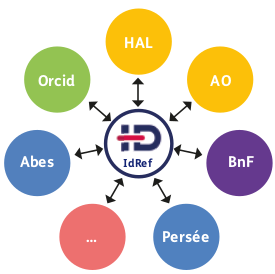
\includegraphics[width=7cm]{images/idref.png}
	\caption[La fédération entreprise par \ac{idref}]{La fédération entreprise par \ac{idref} [Source: \cite[p.9]{aymonin_arabesques_2017}]}
	\label{idref_schema}
\end{figure}

\index[ref]{lod@Linked Open Data (LOD)!viaf@VIAF}\index[ref]{autorites@Autorités!viaf@VIAF}\ac{viaf}, \index[ref]{lod@Linked Open Data (LOD)!idref@IDREF}\index[ref]{autorites@Autorités!idref@IDREF}\ac{idref} ou \index[ref]{lod@Linked Open Data (LOD)!lcsh@LCSH}\index[ref]{autorites@Autorités!lcsh@LCSH}\ac{lcsh} sont quelques uns de ces hubs de liens qui fournissent en une seule page plusieurs identifiants. \ac{idref} est basé sur les autorités du Sudoc, mais a été créé pour effectuer l'interopérabilité entre les différents catalogues du milieu de la recherche à travers un référentiel commun\footnote{\og Il s’agissait de montrer la fonction de pivot des identifiants et les bénéfices d’un adossement des catalogues à un référentiel commun.\fg{} in \cite[p.9]{aymonin_arabesques_2017}}. Ainsi, de multiples référentiels sont liés avec \ac{idref} par leur identifiant~(\reference{idref_schema}): \index[ref]{lod@Linked Open Data (LOD)!rameau@RAMEAU}\index[ref]{autorites@Autorités!rameau@RAMEAU}\ac{rameau} est utilisé, de même que HAL pour les publications scientifiques ouvertes ou Persée; les identifiants \ac{viaf} et \ac{isni} sont également renseignés, \dots


\subsection{\label{III-A-2-c}Les hubs de liens et d'identifiants réceptacles de données}
\titreEntete{Les hubs de liens et d'identifiants réceptacles de données}

\begin{citationLongue}
	D’un hub de références, Wikidata tend à devenir un réceptacle des données elles-mêmes\footcite{poupeau_au-a_2018}.
\end{citationLongue}
\medskip

Le projet \index[ref]{lod@Linked Open Data (LOD)!wikidata@Wikidata}Wikidata est né en 2012 de la volonté de centraliser les informations des Wikipédias sous la forme de données structurées en déclarations. Ce modèle de données ressemble à \index[ref]{echanges@Échanges!formats@Formats!rdf@RDF}\ac{rdf}, mais reste différent en raison des informations supplémentaires apportées par le modèle Wikidata: l'ajout de références et de qualificatifs enrichit les données. Wikidata s'impose dans le Web de données par ses atouts: ses données, augmentées par une communauté imposante, sont disponibles immédiatement et ne dépendent pas des mises à jour --- comme cela était le cas avec \index[ref]{lod@Linked Open Data (LOD)!dbpedia@DBpédia}DBpédia ---; les données de Wikidata se requêtent avec \index[ref]{echanges@Échanges!protocoles@Protocoles!sparql@SPARQL}\ac{sparql}.\\

Premièrement, Wikidata est un hub d'identifiants, de liens. Ces identifiants font l'objet, sur les pages d'entités de Wikidata, d'une partie à part, à la fin de cette page. Ils sont néanmoins de simples déclarations propriété--valeur avec une possibilité d'ajouter des qualificatifs et des références\footnote{Un compte Twitter, qui a un identifiant et qui peut par conséquent faire l'objet d'une déclaration dans une entité de Wikidata, a, par exemple, comme qualificatif le nombre d'abonnés à une date donnée.}.
L'ensemble --- plusieurs centaines --- des propriétés d'identifiants est répertorié sur la page de liste de ces propriétés \href{https://www.wikidata.org/wiki/Wikidata:List_of_properties/Wikidata_property_for_an_identifier}{Wikidata:List of properties/Wikidata property for an identifier}: les jeux de données et les référentiels étant de plus en plus nombreux sur le Web, ces propriétés permettent de typer et de décrire chaque relation avec un identifiant.\\

Deuxièmement, \index[ref]{lod@Linked Open Data (LOD)!wikidata@Wikidata}Wikidata est un réceptacle de données. En effet, en plus des identifiants, Wikidata propose des déclarations structurées biographiques ou générales sur l'entité. En cela, si \index[ref]{lod@Linked Open Data (LOD)!idref@IDREF}\index[ref]{autorites@Autorités!idref@IDREF}\ac{idref} et Wikidata semblaient être similaires avec l'offre de liens, ils diffèrent par cette structuration permanente des informations. Ainsi,  le concept \nP{Vincent}{Dedienne} de \ac{idref}\footnote{\nP{Vincent}{Dedienne} dans \ac{idref}: \url{https://www.idref.fr/196914183}\\\nP{Vincent}{Dedienne} dans Wikidata: \url{https://www.wikidata.org/wiki/Q18413745}} structure l'état civil et les dates, mais met le reste des informations en note: \og Comédien,auteur , acteur et humoriste français\fg{}. Wikidata apporte du sens grâce à la propriété P106 qui permet d'indiquer que la déclaration concerne l'\textit{occupation} de la personne, et d'offrir un lien vers l'entité de cette occupation.\\

Par la structuration de ses données et l'apport de multiples identifiants et liens vers d'autres jeux de données et référentiels, \index[ref]{lod@Linked Open Data (LOD)!wikidata@Wikidata}Wikidata devient un \textit{super} hub, se plaçant plus haut encore que ceux évoqués précédemment.

%conclu
\bigskip
\bigskip
L'agrégation de liens et d'identifiants est un enjeu essentiel de manière à n'effectuer des opérations d'alignement qu'une seule fois, et ainsi diminuer le coût de ces opérations. Ces agrégations nécessitant elles-mêmes des identifiants pour pouvoir exister sur le Web de données, des données structurées sont venues s'ajouter à la simple exposition de liens vers d'autres référentiels. Ainsi, Wikidata a montré son efficacité et se place aujourd'hui comme acteur principal d'agrégation de connaissances et de liens vers d'autres sources de données souvent plus spécialisées.
\section{\label{III-A-3}Wikidata comme hub de liens: aligner les fictions et les séries de l'INA avec Wikidata}
\titreEntete{Wikidata comme hub de liens}

%intro
Le principal intérêt de Wikidata, nous l'avons évoqué précédemment, est l'agrégation de liens et d'identifiants d'autres référentiels et jeux de données. Cela permet d'accéder à un même endroit à divers identifiants de référentiels, sans avoir à effectuer un alignement avec chacun de ces référentiels. L'opération d'alignement de fictions et de séries avec Wikidata ne peut s'effectuer qu'à partir des titres: alors qu'un alignement de personnes se réalise sur un voire deux mots de l'état civil, celui de titres et de séries doit se réaliser sur l'ensemble des mots de ces titres, ce qui augmente considérablement les échecs d'alignement.\\

Cependant, malgré les difficultés, imposées une nouvelle fois par le langage naturel, l'alignement reste une opération importante pour l'enrichissement des données d'une institution: le parcours de liens devient alors possible, et l'accès au Web de données apporte de nouvelles informations sur les instances alignées.

\subsection{\label{III-A-3-a}Enrichir ses données avec des identifiants plutôt qu'avec des textes}
\titreEntete{Enrichir ses données avec des identifiants}

L'établissement de liens avec des référentiels externes est essentiel à l'\ac{ina}. En effet, les données issues du \ac{dl} sont parfois sommaires et tournées vers l'événement de diffusion au détriment de la description documentaire. Si les données achetées à l'extérieur --- auprès de Plurimédia, Médiamétrie, \dots --- apportent les informations les plus importantes, l'ensemble des acteurs d'une série ou d'une fiction ne sont par exemple pas présents dans les bases de données de l'\ac{ina}.\\

Une première possibilité serait alors d'aligner les fictions et les séries avec Wikidata afin de récupérer les libellés des valeurs de la propriété P161 qui permet la déclaration de membres du casting. Cette possibilité nécessiterait néanmoins une mise à jour régulière avec un nouveau lancement de l'alignement, de manière à avoir les données et les informations actualisées de Wikidata. De plus, l'introduction de ces textes coupe les liens qui étaient présents sur Wikidata, et empêche ainsi de naviguer de lien en lien depuis un membre de casting, par exemple, pour arriver sur une autre de ses fictions.\\

Le stockage du seul identifiant de l'entité Wikidata de la fiction ou de la série suffit alors. À partir de cet identifiant, il devient possible d'accéder à toutes les déclarations de l'entité, qu'elles soient biographiques ou générales, ou bien qu'elles soient des liens, ainsi qu'aux déclarations des valeurs de ces déclarations, \dots~ L'alignement des fictions et des séries de l\ac{ina} vise apr conséquent à récupérer les identifiants Wikidata des fictions, des séries, et des épisodes de séries.\\

Parallèlement à cette récupération d'identifiants Wikidata, il est également nécessaire d'obtenir l'\ac{isan}, l'identifiant international de tout document audiovisuel. Cet \ac{isan} permet alors d'obtenir par rebond des informations plus précises sur la fiction ou la série grâce à une base de données spécifique, IMDb\footcite{noauthor_imdb_nodate}. Le stockage à l'\ac{ina} de simples identifiants --- Plurimédia, Médiamétrie, IMédia, Wikidata et \ac{isan} --- est alors suffisant pour avoir accès au Web de données et à l'ensemble des informations et des données disponibles sur ces instances.

\subsection{\label{III-A-3-b}Aligner des fictions et des séries avec Wikidata}
\titreEntete{Aligner des fictions et des séries avec Wikidata}

De même que l'alignement des personnes physiques avec Wikidata\footnote{Voir \reference{II-C}.}, le \ac{sparql}-EndPoint et l'\ac{api} Wikibase sont conjointement utilisés. Une première étape nécessite la récupération de l'ensemble des sous-classes des entités \textit{Film} (Q11424)\footnote{Film (Q11424): \url{https://www.wikidata.org/wiki/Q11424}} et \textit{Série Télévisée} (Q5398426)\footnote{Série Télévisée (Q5398426): \url{https://www.wikidata.org/wiki/Q5398426}} par une requête \ac{sparql} (\reference{sparql_1}).
\begin{figure}[!h]
	\centering
	\begin{minted}{sparql}
select ?serie ?serieLabel
where{
?serie wdt:P279* wd:Q5398426.
service wikibase:label{bd:serviceParam wikibase:language "fr,en"}
}
	\end{minted}
	\caption{Requête \ac{sparql} pour récupérer les sous-classes de l'entité \textit{Série Télévisée}}
	\label{sparql_1}
\end{figure}
Dans le cas des séries télévisées, d'autres entités, non présentes dans la requête de la \reference{sparql_1}, sont nécessaires pour avoir accès à l'ensemble des séries télévisées de Wikidata. Il est ainsi nécessaire de faire une seconde requête avec la propriété P361 qui indique qu'une entité est \og une partie d'\fg{}une autre entité: l'entité de la \textit{saison} (Q3464665)\footnote{Saison (Q3464665): \url{http://www.wikidata.org/entity/Q3464665}}, essentiel dans l'alignement, est récupéré par ce moyen.\\

La récupération des instances de chacune des sous-classes est ensuite possible par une requête \ac{sparql}\footnote{Le \ac{sparql}-EndPoint est ici utilisé en raison du faible nombre de requêtes qui seront effectuées, et du nombre de résultats par requête relativement faible (inférieur à 200000) n'induisant pas de \textit{timeout}.} (\reference{sparql_2}). L'objectif de cette étape n'est pas de récupérer l'ensemble des valeurs des propriétés qui permettent l'alignement --- ce qui ne serait pas possible en raison des limites du \ac{sparql}-EndPoint évoquées au \reference{II-C} ---, mais d'obtenir les identifiants de toutes les entités instances des sous-classes.
\begin{figure}[!h]
	\centering
	\begin{minted}{sparql}
select ?saison ?saisonLabel
where{
?saison wdt:P31 wd:Q3464665.
service wikibase:label{bd:serviceParam wikibase:language "fr,en"}
}
	\end{minted}
	\caption{Requête \ac{sparql} pour récupérer les identifiants des instances de la classe \textit{Saison}}
	\label{sparql_2}
\end{figure}

L'\ac{api} Wikibase, avec le module \textit{wbgetentities} permet ensuite d'obtenir les points de comparaison avec les données de l'\ac{ina}:
\begin{itemize}
	\item pour les fictions, les valeurs suivantes sont ainsi récupérées:
	\begin{itemize}
		\item P577 pour la date de publication de la fiction
		\item P57 pour le réalisateur
		\item P162 pour le producteur
		\item les libellés préférentiels et alternatifs du titre et des noms de personnes sont également ajoutés
	\end{itemize}
	\item pour les séries, plus précisément les épisodes, les suivantes:
	\begin{itemize}
		\item P577 pour la date de publication de l'épisode
		\item P179 pour la série d'appartenance de l'épisode
		\item le qualificatif P1545 de P179 pour le numéro de l'épisode
		\item P4908 pour le nom de la saison
		\item le qualificatif P1545 de P4908 pour le numéro de la saison
		\item les libellés préférentiels et alternatifs des titres sont récupérés en français et en anglais --- en effet, un grand nombre de séries conservées à l'\ac{ina} n'ont pas de titres traduits
		\item les libellés préférentiels et alternatifs des valeurs des propriétés sont récupérés uniquement en français
	\end{itemize}
\end{itemize}

Cette récupération de différentes données permet un alignement avec les données de l'\ac{ina}. La fiction long métrage \og Doux dur et dingue\fg{} de \nP{James}{Fargo} en 1978 trouve ainsi son entité équivalente (\href{https://www.wikidata.org/wiki/Q1195524}{Q1195524}) dans Wikidata grâce à une stricte égalité --- après passage des majuscules en minuscules et suppression de la ponctuation --- des titres: l'\ac{isan} (déclaré avec la propriété P3212) \og 0000-0000-3B9A-0000-D-0000-0000-Z\fg{} peut alors être ajouté aux données de l'\ac{ina} en plus de l'identifiant Wikidata.
Pour les séries, ce sont les épisodes qui subissent l'alignement car chacun d'entre eux est identifié individuellement et lié ensuite avec sa série d'appartenance: le troisième épisode de la comédie de situation \og 3ème planète après le Soleil\fg{}, \og The Fifth Solomon\fg{}, est alors aligné doublement. Il l'est une première fois avec sa série (\href{https://www.wikidata.org/wiki/Q870490}{Q870490}), et une seconde fois avec son entité équivalente dans Wikidata, \href{https://www.wikidata.org/wiki/Q18040623}{Q18040623}. Enfin, l'\ac{isan}, quand il est disponible, est également ajouté, ce qui est le cas pour cet épisode identifié internationalement par l'identifiant \og 0000-0001-637C-0065-4-0000-0000-P\fg{}.

\subsection{\label{III-A-3-c}Les difficultés posées par les langages naturels}
\titreEntete{Les difficultés posées par les langages naturels}

Les résultats obtenus après un alignement de fictions ou de séries avec Wikidata peuvent paraître faibles: si les fictions sont alignées presque à 50\%, ce n'est pas le cas des séries pour lesquelles à peine 10\% des épisodes ont pu être alignés avec leur équivalent Wikidata. Bien que de nombreux épisodes et séries n'existent pas sur Wikidata, comme \og Mon père dort au grenier\fg{} dont il existe 26 saisons, cette absence d'entités Wikidata n'est pas suffisante pour expliquer les faibles alignements des séries.\\

La raison principale est le langage naturel utilisé de chaque côté de l'alignement, et les nombreuses divergences de graphie qui peuvent exister sur les mots des titres. En effet, les titres des séries sont pour certains traduits en français, d'autres restent en anglais, à la fois dans les données de l'\ac{ina} et sur Wikidata. L'alignement n'utilisant pas de traducteur ou d'intelligence artificielle, la similarité entre, par exemple, l'instance de l'\ac{ina} \og Monk va à la noce\fg{} de la saison 7 de Monk, avec l'entité \href{https://www.wikidata.org/wiki/Q50846176}{Q50846176} \og Mr. Monk Goes to a Wedding\fg{} qui lui correspond. L'alignement n'aura alors réussi à aligner que la série d'appartenance (Q189068) de cet épisode, et non l'épisode lui-même. L'utilisation des libellés préférentiels et alternatifs en français et en anglais aura, ici, été inutile. Cependant, la prise en compte de l'anglais a permis de nombreux alignements d'épisodes qui, tant du côté de l'\ac{ina} que de Wikidata, n'ont pas été traduits.\\

De plus, des séries très longues, comme \og Amour, gloire et beauté\fg{}, qui compte plus de 5000 épisodes, peuvent ne pas être décrites dans Wikidata au niveau de l'épisode. Quand une entité d'épisode est disponible dans Wikidata et que ce titre ne correspond pas à celui de l'\ac{ina}, il est possible d'utiliser le numéro de saison et d'épisode pour effectuer l'alignement. Seulement, le comptage des épisodes est différent selon Wikidata et l'\ac{ina}: Wikidata ne réinitialise pas le numéro d'épisode au début de chaque saison, alors que l'\ac{ina} le fait le plus souvent.\\

Les difficultés à l'alignement des fictions et des séries sont multiples, ce qui entraîne un faible rendement, notamment quand il s'agit d'aligner à la fois un libellé et un autre libellé d'une valeur de déclaration. Les graphies et les langues varient énormément. Les limites d'un alignement par stricte égalité sur des textes sont certainement ici atteintes. Des méthodes alternatives seraient nécessaires comme l'utilisation d'un traducteur puis de réseaux de neurones permettant d'aligner sur des similarités de textes et des égalités de numéro de saison ou de producteur.

%conclu
\bigskip
\bigskip
Bien que nécessaire, la récupération d'identifiants et de liens sur le Web de données, principalement sur Wikidata, peut se révéler difficile selon le type de données permettant l'alignement, et le genre des entités et des instances. L'alignement de personnes, effectué sur peu de mots et des données structurées comme les dates, est ainsi plus facile à réaliser que l'alignement de séries qui ne peut se faire qu'à partir d'une longue chaîne de caractères, le titre.

%conclu
\bigskip
\bigskip
\bigskip
Le succès des modèles de données en graphe est incontestable et est repris dans tous les projets d'envergure internationale: nous avons évoqué Wikidata, le projet European Holocaust Research Infrastructure (EHRI)\footnote{Site du projet: \cite{noauthor_european_nodate}\\Utilisation du graphe de données: \cite{blanke_developing_2015}} peut également être cité comme acteur institutionnel se dégageant des bases de données relationnelles et des traditionnels référentiels hiérarchiques et contrôlés. Cependant, ce modèle de graphe nécessite un langage de requête efficace et des rendements élevés. Or, il a été constaté avec Wikidata et le \ac{sparql}-EndPoint des lenteurs de retours de résultats, obligeant à utiliser d'autres moyens pour obtenir les entités de Wikidata avec leurs déclarations.\\

La recentralisation des données autour de quelques acteurs du Web de données est une conséquence inattendue de la décentralisation de ces mêmes données qui avait eu lieu quelques années auparavant avec la publication de jeux de données et de référentiels sur le Web sémantique. Cette recentralisation est née d'un besoin d'obtenir en un même endroit une multiplicité de liens, d'identifiants et d'informations, sans avoir à connaître les institutions ou les jeux de données dans lesquels aller chercher les données nécessaires. Si cette recentralisation concerne ici le Web de données, elle peut également concerner les institutions directement, ainsi que les entreprises: on ne parle alors plus de Linked Open Data, mais de Linked Enterprise Data (LED).